\section{نسخه نخست مدل و دلیل کارنکردن آن روی داده جدید}
\label{app:ch3-first}
مدل فصل~\ref{ch:tagger} را با همان تنظیم‌ها (جدول~\ref{tab:ch3-diff}، ستون فصل ۱) روی داده‌های شبیه‌سازی‌شده فصل~\ref{ch:data} آموزش دادیم و آن را «نسخه نخست» می‌نامیم. این پیوست نتایج آن و دلیل کار نکردنش را می‌آورد، که به اصلاح ورودی و آموزش و رسیدن به \lr{QGNN+} (فصل~\ref{ch:train}) انجامید.

\subsection{نتایج نسخه نخست}
نسخه نخست روی \lr{jetImage} خوب کار می‌کند: \lr{AUC} آزمون برابر $0.886\pm0.017$ است (۳ بذر تصادفی). در یکی از بذرهای تصادفی \lr{AUC} در دوره‌های ۶ تا ۱۷ تا حدود ۰٫۵ پایین می‌آید و دوباره بهبود می‌یابد. روی \Zjet در برابر \bbbb وضع بسیار بدتر است: \lr{AUC} برابر $0.638\pm0.020$ (بذرهای تصادفی: \lr{0.629}، \lr{0.661}، \lr{0.625}). آموزش و اعتبارسنجی نزدیک هم می‌مانند، پس این کار ذاتاً دشوارتر از \Zbos{} در برابر گلوئون است (شکل‌های~\ref{fig:ch3-step1} و~\ref{fig:ch3-step2}).

\begin{figure}[H]
\centering
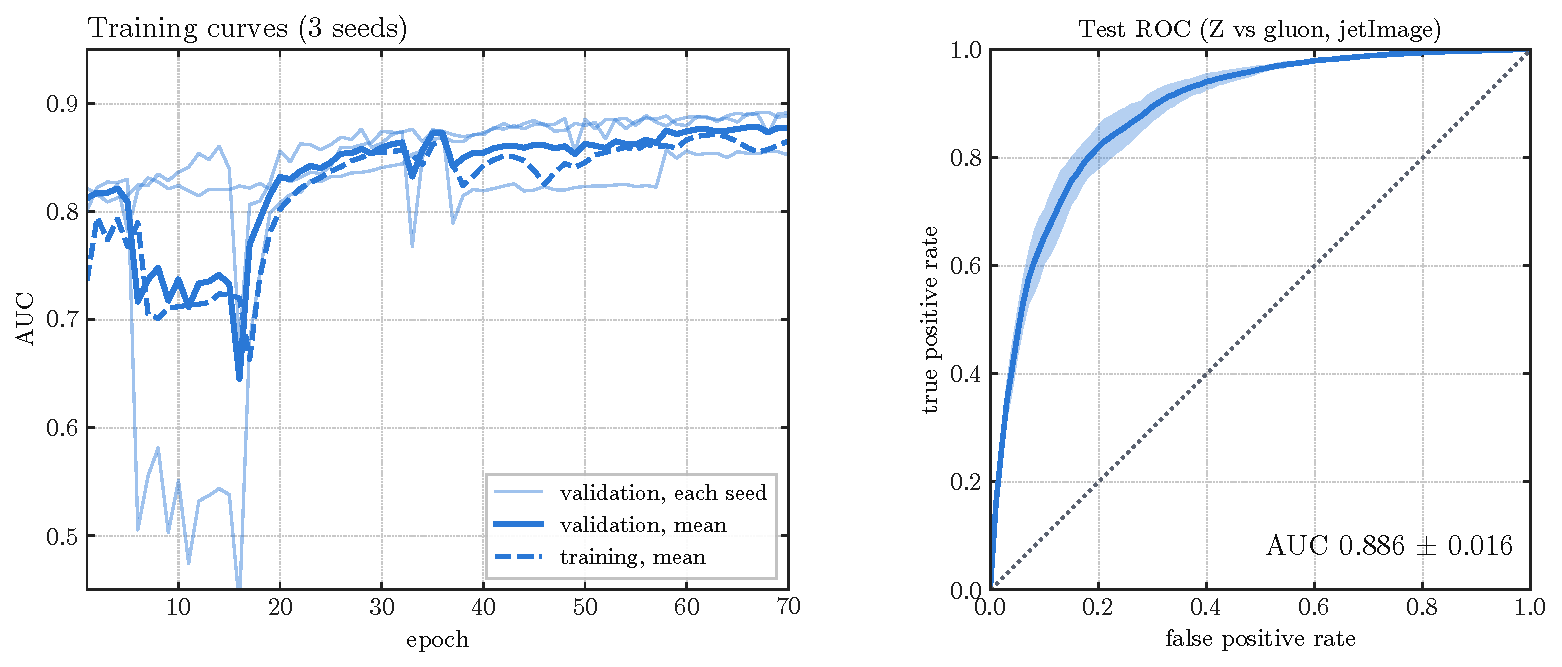
\includegraphics[width=\textwidth]{figs/ch3_step1.pdf}
\caption{منحنی‌های آموزش (چپ: \lr{AUC} آموزش و اعتبارسنجی در هر دوره) و منحنی \lr{ROC} آزمون (راست، میانگین ۳ بذر تصادفی با نوار \lr{$\pm$}یک انحراف معیار) نسخه نخست روی \lr{jetImage}.}
\label{fig:ch3-step1}
\end{figure}

\begin{figure}[H]
\centering
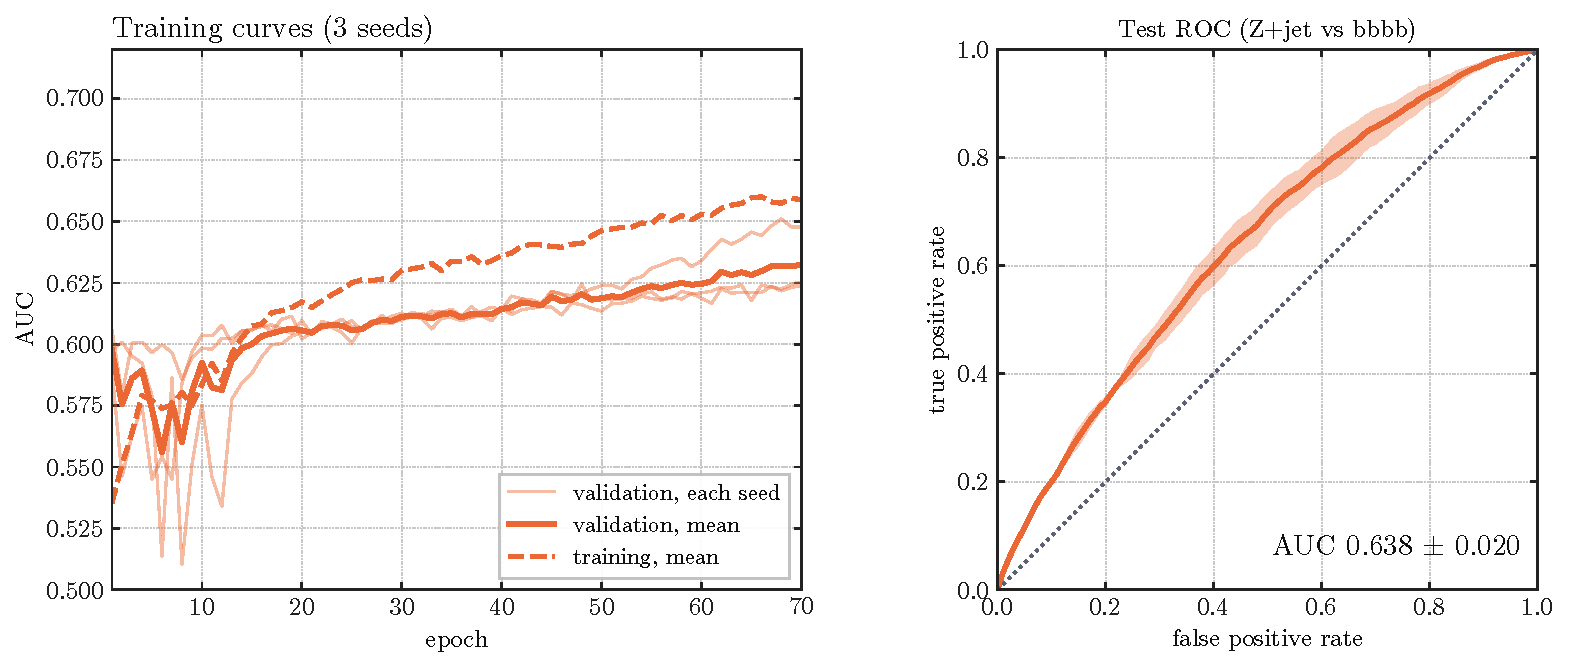
\includegraphics[width=\textwidth]{figs/ch3_step2.pdf}
\caption{همان شکل~\ref{fig:ch3-step1} برای \Zjet در برابر \bbbb. مدل در این مسئله بسیار ضعیف‌تر است.}
\label{fig:ch3-step2}
\end{figure}

وقتی این دو شناساگر روی جت‌های \ttZ و \ttbb، که در آموزش نبوده‌اند، امتیاز می‌دهند، هر دو نزدیک شانس‌اند: شناساگر \lr{jetImage} \lr{AUC} برابر $0.524\pm0.016$ و شناساگر \Zjet در برابر \bbbb برابر $0.579\pm0.028$ می‌دهد، یعنی کمتر از \lr{0.638} خودش روی آزمون خودش (جدول~\ref{tab:ch3-exps} و شکل~\ref{fig:ch3-ttzttbb}).

\begin{figure}[H]
\centering
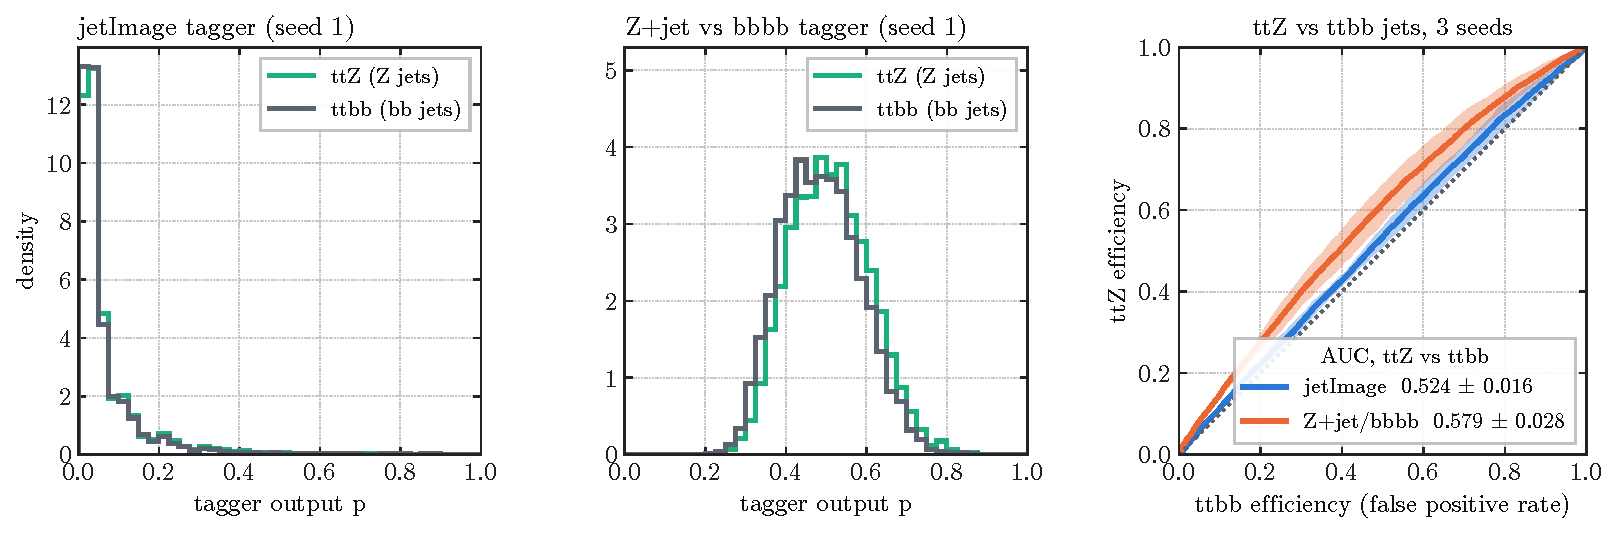
\includegraphics[width=\textwidth]{figs/ch3_ttz_ttbb.pdf}
\caption{امتیاز دو شناساگر نسخه نخست روی جت‌های \ttZ و \ttbb که در آموزش نبوده‌اند: توزیع امتیاز (دو شکل چپ) و منحنی \lr{ROC} (راست، ۳ بذر تصادفی با نوار \lr{$\pm$}یک انحراف معیار).}
\label{fig:ch3-ttzttbb}
\end{figure}

\begin{table}[H]
\centering
\caption{آنچه آموزش دیده و آنچه روی آن به کار رفته است. \lr{AUC} روی مجموعه آزمون؛ ۳ بذر تصادفی برای هر مدل.}
\label{tab:ch3-exps}
\begin{tabular}{p{3.2cm}p{3.6cm}c p{3.8cm}c}
\toprule
مدل & آموزش‌دیده روی & \lr{AUC} آزمون خودش & به‌کاررفته روی & \lr{AUC} آنجا \\
\midrule
\lr{QGNN} نسخه نخست & \lr{jetImage} & \lr{0.886} & جت‌های \ttZ و \ttbb & \lr{0.524} \\
\lr{QGNN} نسخه نخست & \Zjet در برابر \bbbb & \lr{0.638} & جت‌های \ttZ و \ttbb & \lr{0.579} \\
\lr{QGNN+} & \Zjet در برابر \bbbb & \lr{0.866} & جت اول رویدادهای \ttZ و \ttbb & \lr{0.793} \\
شبکه گرافی کلاسیک (تنظیم پیش‌فرض) & \Zjet در برابر \bbbb & \lr{0.861} & جت اول رویدادهای \ttZ و \ttbb & \lr{0.787} \\
\bottomrule
\end{tabular}
\end{table}


\subsection{مقایسه با مدل‌های کلاسیک روی ورودی نخست}
برای دانستن اینکه مدار کوانتومی چیزی می‌افزاید یا نه، همان کار را با مدل‌های کلاسیک انجام دادیم (جدول~\ref{tab:ch3-base}). شبکه گرافی کلاسیک همان رمزگذار و همان گراف نهان را دارد و به‌جای مدار از انتقال پیام استفاده می‌کند، و فقط با آنتروپی متقاطع دودویی آموزش می‌بیند. اندازه پنهان ۴ (۷۷ پارامتر) و ۳۲ (۲۴۰۱ پارامتر) \lr{AUC} یکسانی می‌دهند. \lr{BDT} و \lr{MLP} ورودی $10\times160$ را مسطح‌شده می‌خوانند. جت‌ها و تقسیم داده برای همه مدل‌ها یکی است. شبکه گرافی کلاسیک با \lr{AUC} برابر $0.631$ از \lr{QGNN} ($0.638$) فرقی ندارد، پس مدار هیچ سودی نداده است.

\begin{table}[H]
\centering
\caption{مقایسه \lr{QGNN} نسخه نخست با مدل‌های کلاسیک روی ورودی نخست. \lr{BDT} و \lr{MLP} یک اجرا هستند و \lr{$\pm$} انحراف معیار روی بذرهای تصادفی است (شبکه گرافی کلاسیک: ۶ اجرا).}
\label{tab:ch3-base}
\begin{tabular}{lcc}
\toprule
مدل & \lr{AUC} روی \Zjet در برابر \bbbb & \lr{AUC} روی \lr{jetImage} \\
\midrule
\lr{BDT} & \lr{0.678} & \lr{0.902} \\
\lr{MLP} & \lr{0.648} & \lr{0.881} \\
شبکه گرافی کلاسیک & $0.631\pm0.003$ & $0.895\pm0.001$ \\
\lr{QGNN} & $0.638\pm0.020$ & $0.886\pm0.017$ \\
\bottomrule
\end{tabular}
\end{table}


\subsection{چرا ورودی نخست کافی نبود}
ورودی نخست فقط قدر مطلق اختلاف هر همسایه با ذره اصلی را نگه می‌دارد، پس \pt مطلق، انرژی و هر کمیت سطح جت از آن حذف شده است. برای سنجش اهمیت این کمیت‌ها، هر کدام را جداگانه آزمودیم. تعداد ذره‌ها به‌تنهایی \lr{AUC} برابر \lr{0.706} می‌دهد (میانه ۴۰ برای \Zjet و ۵۰ برای \bbbb)، جرم \lr{0.527} و \pt برابر \lr{0.504}. طیف‌های \pt دو نمونه یکسان‌اند و یک \lr{BDT} روی پنج ویژگی سطح جت، یعنی جرم، \pt، تعداد مؤلفه‌ها، \lr{girth} و \lr{$p_\mathrm{T}D$}، که از مؤلفه‌ها محاسبه می‌شوند، در هر چارک \pt مقدار \lr{AUC} را بین \lr{0.83} و \lr{0.88} نگه می‌دارد. در ورودی نخست، یک \lr{BDT} بیشتر از زاویه‌ها ($\cos\theta_\mathrm{rel}$ و $\cos\theta$) و سپس از کسرهای انرژی استفاده می‌کند و هیچ ویژگی تنها بیش از \lr{0.60} نمی‌دهد، پس اطلاعات بین اعداد زیادی پخش است.

ورودی جدید برای هر گره ۱۸۱ عدد دارد: همان ۱۶۰ اختلاف همسایه‌ها، به‌علاوه ۱۶ ویژگی مطلق ذره اصلی و ۵ ویژگی سطح جت (جرم، \pt، تعداد ذره‌ها، \lr{girth} و \lr{$p_\mathrm{T}D$}) که روی هر ده گره تکرار می‌شوند. جت‌های \ttZ و \ttbb با همان ۱۸۱ عدد و همان مقیاس‌دهی ساخته می‌شوند. روی ورودی جدید همه مدل‌های کلاسیک به‌طور چشمگیری بهتر شدند (جدول~\ref{tab:ch3-newin} و شکل~\ref{fig:ch3-ablation}).

\begin{figure}[H]
\centering
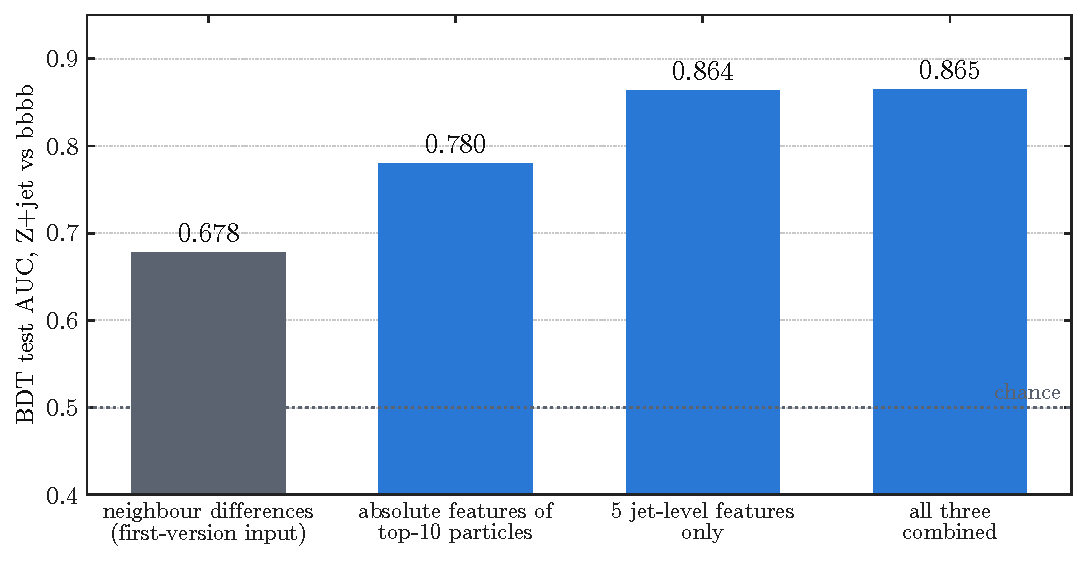
\includegraphics[width=0.7\textwidth]{figs/ch3_ablation.pdf}
\caption{\lr{AUC} آزمون یک \lr{BDT} روی \Zjet در برابر \bbbb با گروه‌های مختلف ورودی. ویژگی‌های سطح جت تنها تقریباً همه تفاوت را می‌سازند.}
\label{fig:ch3-ablation}
\end{figure}

\begin{table}[H]
\centering
\caption{\lr{AUC} روی \Zjet در برابر \bbbb با ورودی نخست (۱۶۰ عدد برای هر گره) و ورودی جدید (۱۸۱ عدد)، با همان جت‌ها و همان تقسیم داده.}
\label{tab:ch3-newin}
\begin{tabular}{lcc}
\toprule
مدل & ورودی نخست & ورودی جدید \\
\midrule
\lr{BDT} & \lr{0.678} & \lr{0.865} \\
\lr{MLP} & \lr{0.648} & \lr{0.851} \\
شبکه گرافی کلاسیک & $0.631$ & $0.861\pm0.007$ \\
\bottomrule
\end{tabular}
\end{table}


\subsection{وارونه شدن \lr{AUC} اعتبارسنجی}
اولین تلاش با \lr{QGNN} روی ورودی جدید شکست خورد: \lr{AUC} اعتبارسنجی وارونه شد. در دو بذر تصادفی \lr{AUC} اعتبارسنجی به \lr{0.84} رسید و در دوره ۸ تا ۱۱ به زیر \lr{0.5} افتاد، در حالی که \lr{AUC} آموزش دوباره بالا آمد. بذر تصادفی سوم هرگز یاد نگرفت (\lr{0.50}). \lr{AUC} آزمون برای سه بذر تصادفی \lr{0.305}، \lr{0.503} و \lr{0.258} بود. \lr{AUC} آموزش با دراپ‌اوت روشن و \lr{AUC} اعتبارسنجی با دراپ‌اوت خاموش محاسبه می‌شود (شکل~\ref{fig:ch3-v2}).

\begin{figure}[H]
\centering
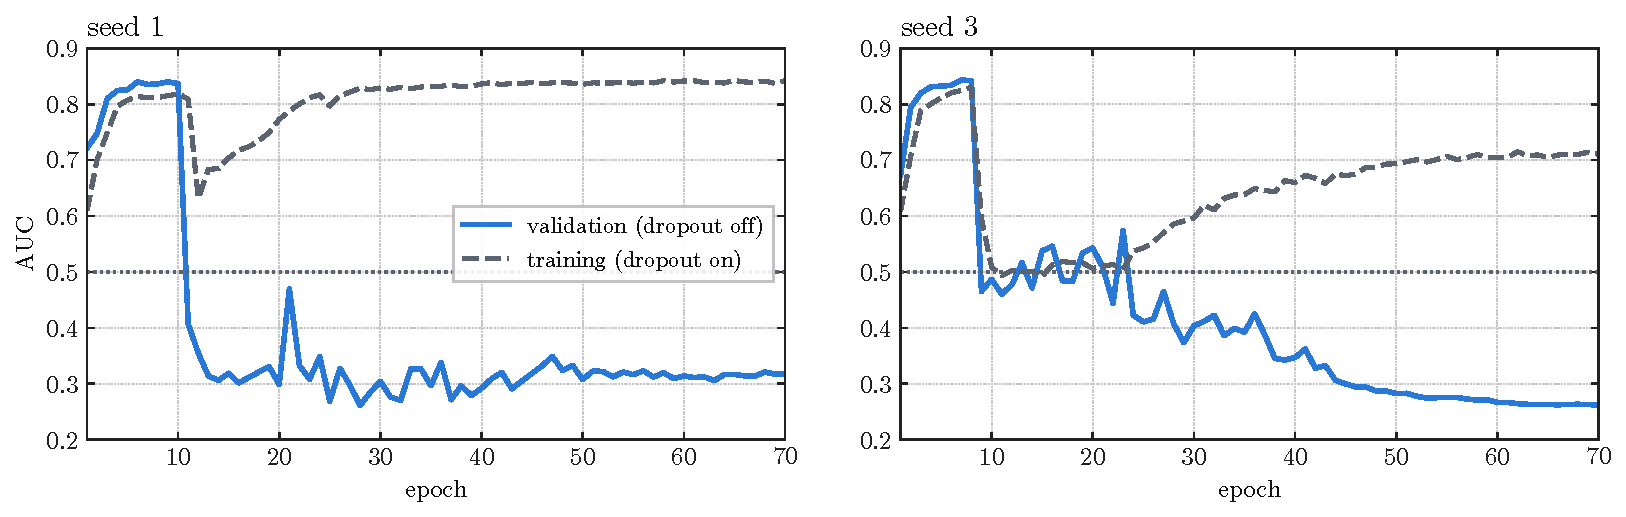
\includegraphics[width=\textwidth]{figs/ch3_v2.pdf}
\caption{وارونه شدن \lr{AUC} اعتبارسنجی (دراپ‌اوت خاموش) در آموزش \lr{QGNN} با ورودی ۱۸۱‌عددی، برای دو بذر تصادفی.}
\label{fig:ch3-v2}
\end{figure}

برای تشخیص دلیل، وزن‌های یک بذر تصادفی را با دراپ‌اوت روشن و خاموش آزمودیم (۱۵۰۰ جت در هر مورد، یک گذر تصادفی). با دراپ‌اوت روشن، \lr{AUC} روی جت‌های آموزش \lr{0.835} و روی جت‌های اعتبارسنجی \lr{0.819} بود، یعنی هم‌سطح شبکه گرافی کلاسیک. با دراپ‌اوت خاموش، همین وزن‌ها \lr{0.316} و \lr{0.334} دادند و ترتیب امتیازها وارونه بود. فرضیه ما این است که گراف نزدیک‌ترین همسایه‌ها از فاصله‌های فضای نهان ساخته می‌شود و این فاصله‌ها با دراپ‌اوت تغییر می‌کنند. آزمایش نشان داد با دراپ‌اوت صفر وارونگی از بین می‌رود.

\section{تعداد پارامترهای مدل‌ها}
\label{sec:ch3-paramsapp}
جدول~\ref{tab:ch3-params} تعداد پارامترهای قابل آموزش هر مدل را در هر مرحله نشان می‌دهد. شمارش‌ها از خود کد آموزش گرفته شده‌اند. برای \lr{QGNN+} رمزگذار (۳۱٬۸۱۲ پارامتر) و مدار (۲۸۱ پارامتر برای هر لایه) شمرده شده‌اند. مولد کمکی گراف (حدود ۴۶ هزار پارامتر) فقط در آموزش، برای تابع هزینه \lr{Sinkhorn}، به کار می‌رود و در پیش‌بینی نقشی ندارد، پس شمرده نشده است. در مرحله رویدادی مدل کوانتومی کوچک است و به‌طور کل ۲٬۰۳۸ پارامتر دارد، یعنی حدود ۱۵ تا ۵۲ برابر کمتر از مدل‌های کلاسیک عمومی (شبکه گرافی، \lr{ParticleNet}‌گونه، \lr{MLP} و ترنسفورمر)، با \lr{AUC} نزدیک (جدول~\ref{tab:ch3-ev3}). کنترل کلاسیک با همان رمزگذار و گراف ۲٬۷۸۹ پارامتر دارد، یعنی تنها حدود ۱٫۴ برابر بزرگ‌تر از مدل کوانتومی. در مرحله جت، رمزگذار ۱۸۱‌ورودی بخش اصلی پارامترها را دارد و مدار تنها ۵۶۲ پارامتر اضافه می‌کند؛ پس در آن مرحله فاصله به مدل‌های \lr{ParT} و \lr{ParticleNet} است که ۱۱ تا ۶۷ برابر بزرگ‌ترند.

\begin{table}[H]
\centering
\caption{تعداد پارامترهای قابل آموزش در هر مرحله. \lr{BDT} پارامتر ندارد و با ۳۰۰ تکرار تقویت ساخته می‌شود.}
\label{tab:ch3-params}
\begin{tabular}{llc}
\toprule
مرحله & مدل & تعداد پارامتر \\
\midrule
جت & \lr{QGNN+}، دو لایه & \lr{32\,374} \\
جت & \lr{QGNN+}، یک لایه & \lr{32\,093} \\
جت & شبکه گرافی کلاسیک (۴ ویژگی پنهان) & \lr{31\,889} \\
جت & \lr{ParticleNet}، ذره‌های خام & \lr{366\,160} \\
جت & \lr{ParticleNet}، ورودی \lr{QGNN+} & \lr{399\,920} \\
جت & \lr{ParT}، ذره‌های خام & \lr{2\,140\,000} \\
جت & \lr{ParT}، ورودی \lr{QGNN+} & \lr{2\,160\,000} \\
\midrule
ویژگی‌های دو جت & \lr{VQC}، ۸ کیوبیت، ۴ لایه & \lr{130} \\
ویژگی‌های دو جت & \lr{VQC}، ۹ کیوبیت، ۴ لایه & \lr{146} \\
ویژگی‌های دو جت & \lr{VQC}، ۱۰ کیوبیت، ۴ لایه & \lr{162} \\
\midrule
ده شیء رویداد & \lr{QGNN} رویدادی & \lr{2\,038} \\
ده شیء رویداد & کنترل کلاسیک (همان رمزگذار و گراف) & \lr{2\,789} \\
ده شیء رویداد & شبکه گرافی & \lr{31\,105} \\
ده شیء رویداد & \lr{ParticleNet}‌گونه & \lr{55\,873} \\
ده شیء رویداد & \lr{MLP} & \lr{85\,249} \\
ده شیء رویداد & ترنسفورمر & \lr{106\,177} \\
\bottomrule
\end{tabular}
\end{table}
